%======================================================================
\section{Further derivations}\label{app:derivations}
%======================================================================

\subsection{Isometry for the compound Poisson integral}

Let $\tilde L_t=L_t-\lambda_Jm_Jt$ be the compensated compound Poisson process. For a
deterministic square-integrable $f$, $\E\int_0^tf(u)\dd\tilde L_u=0$ and
\[
  \E\Bigl[\Bigl(\int_0^tf(u)\dd\tilde L_u\Bigr)^2\Bigr]=\lambda_J\E[J^2]\int_0^tf(u)^2\dd u .
\]
\emph{Proof.} For a step function $f=\sum_kf_k\1_{(u_k,u_{k+1}]}$ the increments of $\tilde L$
over disjoint intervals are independent with mean zero and variance
$\lambda_J\E[J^2](u_{k+1}-u_k)$, so the second moment is
$\lambda_J\E[J^2]\sum_kf_k^2(u_{k+1}-u_k)$. The general case follows by density of step
functions in $L^2$. Writing $\int f\dd L=\int f\dd\tilde L+\lambda_Jm_J\int f\dd u$ gives the mean
and variance used in Proposition~\ref{prop:cet1}, with $f(u)=e^{-\kappa(t-u)}$.

\subsection{Transition of the CET1 process between observation dates}

Conditionally on $C_s$, \eqref{eq:cet1sol} applied on $[s,t]$ gives
\[
  C_t=\theta+(C_s-\theta)e^{-\kappa(t-s)}+\sigma\int_s^te^{-\kappa(t-u)}\dd W_u-\int_s^te^{-\kappa(t-u)}\dd L_u .
\]
Without jumps the transition is Gaussian with mean $m=\theta+(C_s-\theta)e^{-\kappa\Delta}$ and
variance $\sigma^2(1-e^{-2\kappa\Delta})/(2\kappa)$, $\Delta=t-s$, which is \eqref{eq:outrans}.
With jumps it is a Gaussian mixture: conditionally on $k$ jumps at times
$u_1,\dots,u_k$, the mean is shifted by $-\sum_iJ_ie^{-\kappa(t-u_i)}$. The likelihood used in
Section~\ref{sec:calibration} ignores this term. Over a quarter the probability of a jump is
$1-e^{-0.12/4}\approx3\%$, so the Gaussian likelihood treats rare large moves as diffusion,
which biases $\hat\sigma$ upwards slightly and, through the profile likelihood, $\hat\kappa$ in
an ambiguous direction; the 2023Q1 exclusion removes the one large positive move.

\subsection{Profile likelihood}

Differentiating \eqref{eq:loglik} with respect to $\sigma^2$ gives
$\partial\ell/\partial\sigma^2=-\frac{n}{2\sigma^2}+\frac1{2\sigma^4}\sum_k(C_{k+1}-m_k)^2/w_k$,
which vanishes at \eqref{eq:sigmahat}. Substituting back,
\[
  \ell_p(\kappa)=\ell\bigl(\kappa,\hat\sigma(\kappa)\bigr)
  =-\frac n2\Bigl[1+\log\bigl(2\pi\hat\sigma^2(\kappa)\bigr)\Bigr]-\frac12\sum_k\log w_k(\kappa),
\]
a one-dimensional function of $\kappa$. The likelihood ratio statistic for a fixed $\kappa_0$
is $2[\ell_p(\hat\kappa)-\ell_p(\kappa_0)]$, asymptotically $\chi^2_1$.

\subsection{Yield to call and the delta method}

Let $y(V)$ solve $V=\sum_jc_j(1+y/2)^{-2t_j}$ for the bullet cash flows $c_j$ to $T_1$. By the
implicit function theorem
\[
  \frac{\dd y}{\dd V}=-\Bigl[\sum_jc_jt_j(1+y/2)^{-2t_j-1}\Bigr]^{-1}=-\frac{1}{D_{\mathrm{mod}}V},
\]
where $D_{\mathrm{mod}}$ is the modified duration to call. For a zero-recovery bullet to
$T_1$ with a constant hazard $h$, the price is the risk-free price discounted at $r+h$, so the
continuously compounded yield rises one-for-one with the hazard; in the base attribution the
hazard block of $219$bp of hazard produces $231$bp of semi-annual yield-to-call spread, a ratio
of $1.05$ that reflects compounding and the state dependence of the driver. The price
sensitivity $|V_0'|\approx0.08$ points per basis point of hazard is larger than a bullet's,
because it includes the exposure of extended cash flows beyond $T_1$. The delta method for the
implied hazard, \eqref{eq:sehazard}, follows from the same implicit function argument applied
to $V_0(\lambda)=P$.

\subsection{The credit triangle for the CDS reference points}

For a CDS with constant hazard $h$, recovery $R$ and continuous premium $s$, the protection
leg is $(1-R)\int_0^Th e^{-(r+h)u}\dd u$ and the premium leg $s\int_0^Te^{-(r+h)u}\dd u$, so the
par spread is $s=h(1-R)$ and $h=s/(1-R)$. The CDS rows of Table~\ref{tab:ladder} use this
approximation; it ignores the term structure of the hazard, accrued premium on default and
the difference between the standard coupon and the par spread, all of which are small at
these spread levels.

\subsection{Relation of the nested value to the Owen value}

For a game $v$ on $\mathcal N$ with a partition into unions $\{\mathcal H,\mathcal K\}$, the
Owen value of player $j\in\mathcal H$ averages its marginal contribution over all orders in
which the members of each union are contiguous, with both orders of the unions equally
likely \citep{Owen1977}. The nested value of Section~\ref{sec:attribution} restricts these
orders to those in which $\mathcal H$ comes first. It is therefore the Owen value of the game
in which the union order is fixed, and it inherits efficiency, symmetry within unions and
the null-player property. The full Owen value would average the nested value with the
attribution in which the contract block comes first, which values extension on a riskless
bond and is excluded for the reason given in Section~\ref{sec:robust}.


%======================================================================
\section{Numerical diagnostics}\label{app:numerics}
%======================================================================

\paragraph{Monte Carlo error.} Table~\ref{tab:mcerr} reports, for each AT1 on the valuation
date, the path-wise standard deviation of the conditional payoff, the standard error of the
price with $20{,}000$ paths, the sensitivity of the price to the hazard and the implied
standard error of the hazard from \eqref{eq:sehazard}.

\begin{table}[H]
\centering
\begin{tabular}{lccc}
\toprule
 & 6.875\% NC33 & 7.20\% NC36 & 7.45\% NC35 \\
\midrule
Path-wise s.d.\ of conditional payoff (points) & 7.3 & 7.9 & 7.5 \\
Standard error of the price (points) & 0.051 & 0.056 & 0.053 \\
$|\partial V/\partial\lambda|$ (points per bp) & 0.077 & 0.084 & 0.079 \\
Standard error of $\lambda$ (bp) & 0.67 & 0.66 & 0.67 \\
\bottomrule
\end{tabular}
\caption{Monte Carlo error at the implied hazard, $20{,}000$ paths.}
\label{tab:mcerr}
\end{table}

\paragraph{Convergence.} Table~\ref{tab:conv} reports the implied hazards for path counts from
$5{,}000$ to $40{,}000$ with two independent seeds, and for a fortnightly instead of a
monthly grid. The levels vary by about $\pm1$bp across seeds, in line with the standard
errors of Table~\ref{tab:mcerr}. The cross-bond dispersion is much more stable, at
$2.3$--$2.9$bp across all runs, because the three bonds share their random numbers.
Halving the time step changes the hazards by at most $1.6$bp.

\begin{table}[H]
\centering
\begin{tabular}{llccc}
\toprule
Paths & Seed & 6.875\% NC33 & 7.20\% NC36 & 7.45\% NC35 \\
\midrule
5,000 & 11 & 2.213 & 2.193 & 2.196 \\
5,000 & 23 & 2.215 & 2.183 & 2.195 \\
10,000 & 11 & 2.215 & 2.191 & 2.196 \\
10,000 & 23 & 2.216 & 2.195 & 2.201 \\
20,000 & 11 & 2.210 & 2.186 & 2.188 \\
20,000 & 23 & 2.199 & 2.176 & 2.176 \\
40,000 & 11 & 2.215 & 2.184 & 2.190 \\
40,000 & 23 & 2.201 & 2.176 & 2.180 \\
\midrule
20,000, monthly (base) & 7 & 2.211 & 2.185 & 2.187 \\
20,000, fortnightly & 7 & 2.227 & 2.196 & 2.181 \\
\bottomrule
\end{tabular}
\caption{Implied hazards (\%/yr) by number of paths, seed and time step.}
\label{tab:conv}
\end{table}

\paragraph{Analytic moments.} With the base-case parameters,
Proposition~\ref{prop:cet1} gives a stationary CET1 mean of $12.25\%$ and a stationary
standard deviation of $1.17$pp ($0.56$pp from the diffusion alone); the mean jump is $2.2$pp
and its $95$th percentile $4.4$pp. Proposition~\ref{prop:spread} gives a stationary spread
standard deviation of $100$bp and a stationary probability of a negative spread of $0.3\%$.
The half-lives of shocks are $2.0$ years for capital and $1.4$ years for the spread.

\paragraph{Memory.} The conditional estimator stores, per path, the coupon cash flows and the
integrated driver at the coupon dates. Root-finding with closures over these arrays creates
reference cycles that the Python garbage collector does not free promptly; forcing a
collection after each solve keeps the weekly calibration below 1~GB.

%======================================================================
\section{Parameters}\label{app:params}
%======================================================================

\begin{table}[H]
\centering\small
\begin{tabular}{llll}
\toprule
Symbol & Meaning & Value & Source \\
\midrule
$\theta$ & CET1 target & 13\% & BNP strategic plan \\
$\kappa,\sigma$ & CET1 mean reversion, volatility & 0.35, 0.47pp & base case; MLE 0.165, 0.44 \\
$\lambda_J,m_J,\sigma_J$ & stress jumps & 0.12/yr, 2.2pp, 0.5 & EBA 2025 adverse check \\
$b$ & MDA floor & 5.64\% & P1 + P2R (CET1 part) \\
$w_0$ & combined buffer today & 4.79\% & published requirement 10.43\% \\
$\Delta w$ & O-SII step-ups & +0.25pp, 1-Jan-2027 and 2028 & French O-SII framework \\
$\ctrig$ & trigger & 5.125\% & term sheets \\
$a,\bar s,\eta,\rho$ & spread OU & 0.5, 275bp, 100bp, $-0.3$ & sample mean; assumptions \\
$\beta$ & capital premium & 1\% per pp & assumption \\
$\delta$ & reputational tolerance & 0 (base), up to 100bp & Section~\ref{sec:robust} \\
$\xi$ & share price at trigger / today & 0.2 & assumption \\
$R_{\mathrm{T2}},R_{\mathrm{SNP}}$ & recovery at resolution & 20\%, 40\% & Markit conventions \\
$\lambda$ & AT1 hazard today & 2.19\% (average) & implied \\
$\lres$ & hazard priced in Tier~2 & 1.72\% & implied, T2 2035NC34 \\
$\lambda_1,\lambda_2$ & two-piece $\lres$ & 1.40\%, 2.10\% & implied, both Tier~2 \\
$H,\Delta,n$ & horizon, step, paths & 40 years, 1/12, 20,000 & numerical \\
\bottomrule
\end{tabular}
\caption{Parameters of the base case.}
\end{table}

%======================================================================
\section{Data and reproducibility}\label{app:data}
%======================================================================

\paragraph{Data layout.} The repository separates raw Capital IQ exports
(\texttt{data/raw/}, licensed and not redistributed), public reference inputs
(\texttt{data/reference/}: term sheets, the requirement stack and its sources, the EBA stress
test and the FRED curve) and the processed panel built from them (\texttt{data/processed/}).
A single script, \texttt{build\_bnp\_dataset.py}, produces a daily panel of all six bonds with
accrued interest, yield to first call and spread over the FRED curve, together with the CDS,
the share price and the CET1 print available on each date, and a quarterly capital table
with the requirement and its publication date.

\paragraph{Code map.}
\begin{center}
\small
\begin{tabular}{ll}
\toprule
File & Content \\
\midrule
\texttt{processes.py} & CET1 jump-diffusion \eqref{eq:cet1}, trigger times \\
\texttt{instrument.py} & MDA schedule \eqref{eq:mda}, stylised term sheet \\
\texttt{market.py} & dated bonds, \eqref{eq:spread}--\eqref{eq:hazard}, pricing \eqref{eq:cmc},
  implied $\lambda$; Tier~2 \eqref{eq:t2grid}; piecewise hazard \\
\texttt{data.py} & paths, loaders, valuation date \\
\texttt{build\_bnp\_dataset.py} & raw exports to the processed panel \\
\texttt{calibrate\_bnp.py} & CET1 likelihood, weekly implied hazards, cross-section \\
\texttt{capital\_structure.py} & Tier~2/SNP/CDS ladder, recovery sensitivity, weekly split \\
\texttt{spread\_and\_stress.py} & attribution, call analysis, stress, capital delta \\
\texttt{robustness.py} & reputational call, Shapley attributions, term structure \\
\texttt{parameter\_uncertainty.py} & bootstrap of $(\kappa,\sigma)$, $\kappa$ scan \\
\texttt{numerics.py} & Monte Carlo errors, convergence, analytic moments \\
\bottomrule
\end{tabular}
\end{center}

\paragraph{Reproduction.} \texttt{run\_all.sh} rebuilds the panel, runs the test suite
(32 tests, including the reduction of the piecewise hazard to the flat one, the
round trip of the implied resolution hazard and the effect of the call tolerance), and
regenerates every table and figure in about thirty minutes. Dates, levels and annotations in
the figures are read from the data, so newer exports and a new \texttt{VALUATION\_DATE}
update the whole paper.

%======================================================================
\section{Additional figures}\label{app:figures}
%======================================================================

\begin{figure}[H]
\centering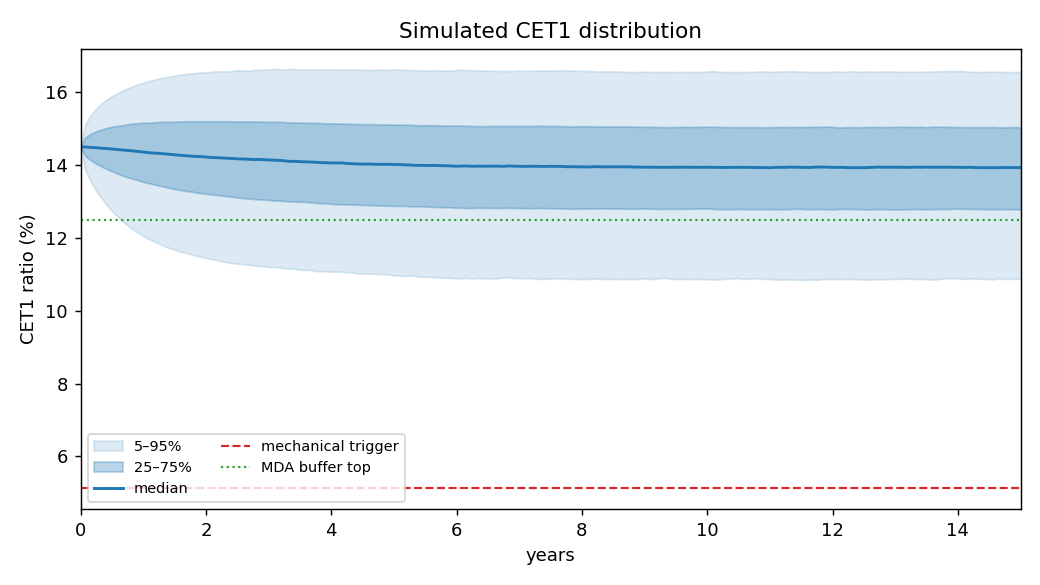
\includegraphics[width=0.75\textwidth]{cet1_fan_chart.png}
\caption{The stylised engine of the repository with illustrative parameters (not the BNP
calibration): simulated CET1 distribution over fifteen years, with the top of the MDA buffer
and the mechanical trigger.}
\end{figure}

\begin{figure}[H]
\centering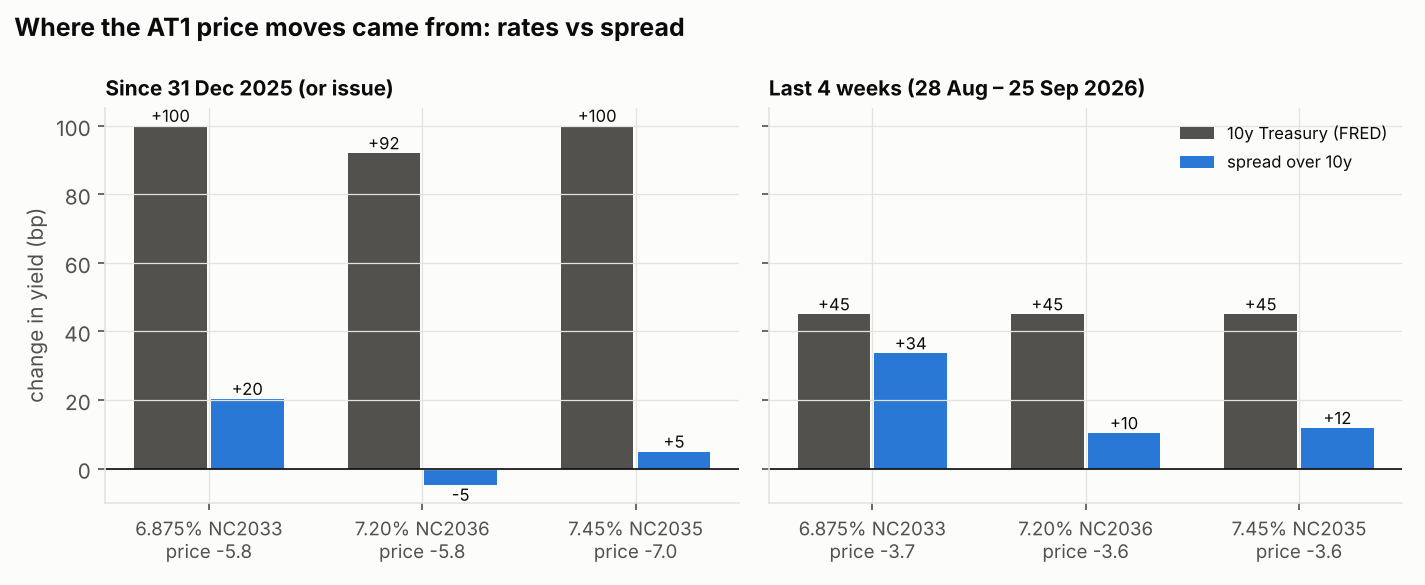
\includegraphics[width=0.85\textwidth]{bnp_at1_yield_split.png}
\caption{Change in each AT1's yield since 31 December 2025 (or issue) and over the four weeks
to 25 September 2026, split into the change in the ten-year Treasury yield and the change in
the spread over it.}
\end{figure}

\begin{figure}[H]
\centering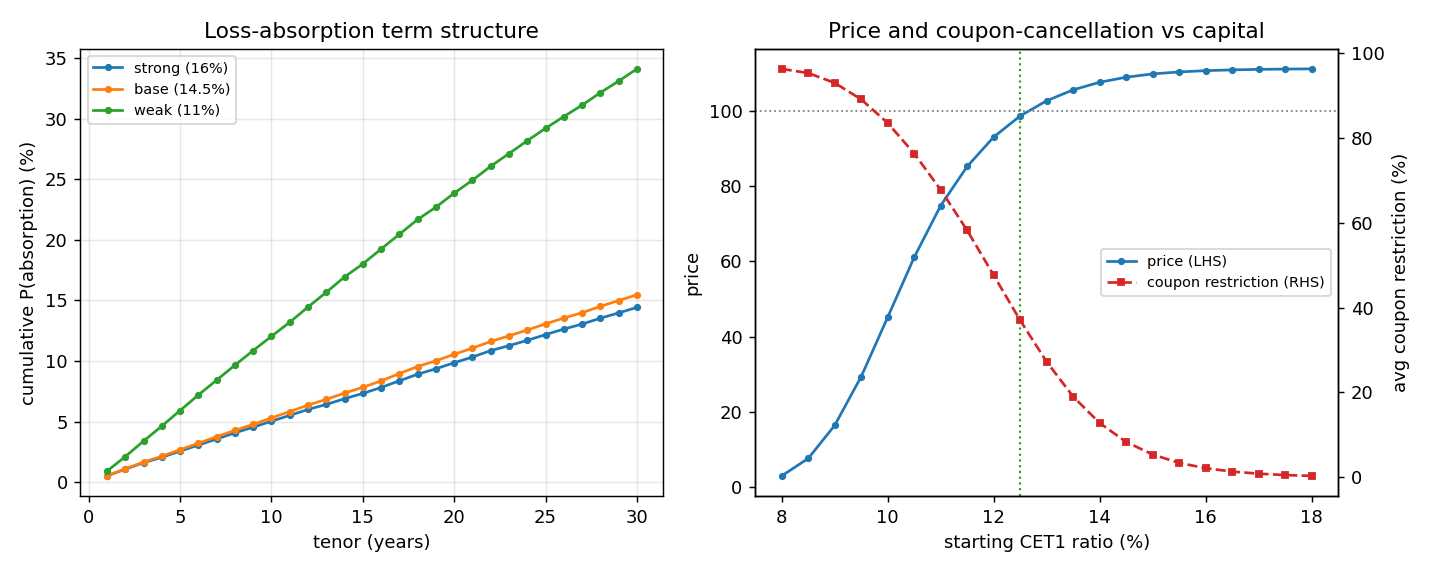
\includegraphics[width=0.85\textwidth]{absorption_and_price_curves.png}
\caption{The stylised engine with illustrative parameters: cumulative probability of loss
absorption by tenor for a strong, base and weak bank (left), and price and average coupon
restriction against the starting CET1 ratio (right).}
\end{figure}
